\documentclass[a4paper,11pt]{article}

% Always keep your main language last
\usepackage[norsk,nynorsk,samin,british]{babel}

\usepackage{_sty/UiT}
\usepackage{_sty/IMS}
\usepackage{MAT-2202/MAT-2202}

% ============================================================ 
% COURSE INFORMATION
% ============================================================

% Default time is 09:00 - 13:00 | Uncomment and change the line below  \visif neccecary
% \newcommand{\examtime}{15:00--19:00}
\newcommand{\location}{\aasgard}
\newcommand{\permittedAids}{%
    \supportMaterial{c,r}}
\newcommand{\paper}{squares}
\newcommand{\pages}{} % Sets the total number of pages manually. Uncomment if neccecary
\newcommand{\contact}{\TrygveJoh}
\newcommand{\mobile}{}
\settoggle{isVisit}{true} % Uncomment this line if examinator / person in charge is visiting
\newcommand{\visitWhen}{ca. kl. 11:00}
\settoggle{showVisit}{false} %Uncomment if unknown when visit

% \newcommand{\ExerciseNumber}{1}

\Published{2017}{09}{26}% YEAR {dddd} MONTH {01 - 12} DAY {01 - 31} 
% \Deadline{2018}{11}{27}% Has to be set, not visible if exam

\settoggle{isLF}{true}
\settoggle{isLF}{false} % Comment this line to show solutions

\settoggle{isEksamen}{false}
\settoggle{isEksamen}{true} % Uncomment this if used for exams

\settoggle{isEksamenUtsatt}{false}
% \settoggle{isEksamenUtsatt}{true} % Uncomment this line if Re sit exam (kont / utsatt eksamen)

% ============================================================ 
% v OWN COMMANDS AND PACKAGES BELOW HERE v
% ============================================================

\usetikzlibrary{decorations.pathreplacing,
decorations.markings,
positioning,
arrows.meta}
\tikzset{
  % style to apply some styles to each segment of a path
  on each segment/.style={
    decorate,
    decoration={
      show path construction,
      moveto code={},
      lineto code={
        \path [#1]
        (\tikzinputsegmentfirst) -- (\tikzinputsegmentlast);
      },
      curveto code={
        \path [#1] (\tikzinputsegmentfirst)
        .. controls
        (\tikzinputsegmentsupporta) and (\tikzinputsegmentsupportb)
        ..
        (\tikzinputsegmentlast);
      },
      closepath code={
        \path [#1]
        (\tikzinputsegmentfirst) -- (\tikzinputsegmentlast);
      },
    },
  },
  % style to add an arrow in the middle of a path
  mid arrow/.style={postaction={decorate,decoration={
        markings,
        mark=at position .55 with {\arrow[#1]{Stealth[scale=1.5]}}
      }}},
}

\begin{document}

\FrontpageUiT[english]

% \include{MAT-2202-Exam-bok-26-09-2017}

% \include{MAT-2202-Exam-nyn-26-09-2017}

\titlebox[english]

Please show work justifying your answers and conclusions.

All ten sub-problems count equally.

\vspace{-0.25cm}
\Problem
    
\begin{subproblem}
    \label{subproblem:MAT-2202-26-09-2017-problem-1a}
    For the function
    %
    \begin{equation}
        f(x_1, x_2) = x_1^4 - x_1 x_2 + x_2^4
    \end{equation}
    %
    find all three stationary points.
\end{subproblem}

\begin{subproblem}
    For the function $f(x_1,x_2)$ in \cref{subproblem:MAT-2202-26-09-2017-problem-1a}, use
    $\vx_0 = (1, 1)$ as the initial point for a gradient search with constant step size $\alpha = \num{0.1}$, to calculate the iterate $\vx_1$.
\end{subproblem}

\begin{subproblem}
    \label{subproblem:MAT-2202-26-09-2017-problem-1c}
    For the function $f(x_1, x_2)$ in \cref{subproblem:MAT-2202-26-09-2017-problem-1a}, use
    $\widetilde{x}_0 = (1,1)$ as the initial point for a 
    Newton search, to calculate the iterate $\widetilde{x}_1$. 
\end{subproblem}

\begin{subproblem}
    Is the Newton step in \cref{subproblem:MAT-2202-26-09-2017-problem-1c} a descent direction?
\end{subproblem}

\vspace{-0.25cm}
\Problem

\begin{subproblem}
    \label{subproblem:MAT-2202-26-09-2017-4a}
    The linear program
    %
    \begin{align*}
        \phantom{2}x_1 + 2 x_2 + 4x_3 \to &\min \\
        4x_1 + \phantom{2}x_2 + 2x_3 \geq{}&{}3 \\
        2x_1 + 4x_2 + \phantom{4}x_3 \geq{}&{}5 \\
        x_1, x_2,x_3 \geq{}&{}0 
    \end{align*}
    %
    is in canonical form. Write down its dual linear program, and solve the dual.
    (Find an optimal solution and the corresponding optimal value).
\end{subproblem}

\begin{subproblem}
    \label{subproblem:MAT-2202-26-09-2017-4b}
    Writing down the linear program in \cref{subproblem:MAT-2202-26-09-2017-4a} in standard form
    %
    \begin{alignat*}{2}
        \phantom{2}x_1 + 2 x_2 + 4x_3 && \to &\min \\
        4x_1 + \phantom{2}x_2 + 2x_3 &&{}- e_1 \geq & \ 3 \\
        2x_1 + 4x_2 + \phantom{4}x_3 &&{}- e_2 \geq & \ 5 \\
        x_1, x_2,x_3,e_1,e_2 &&  \geq & \ 0 
    \end{alignat*}
    %
    Check that $\vx = \mat{0&1&1&0&0}\tran$ is a basic feasible solution. Establish that it is not an optimal solution.
\end{subproblem}

\begin{subproblem}
    Perform a single step of the simplex method
    to obtain from the vector $\vx = \mat{0&1&1&0&0}\tran$ a new basic feasible solution
    of the LP problem in
    \cref{subproblem:MAT-2202-26-09-2017-4b}
    that improves the objective.
\end{subproblem}

\begin{subproblem}
    The figure below shows a road network from A to F,
    with four toll booths at B, C, D and E. To pass each booth
    it is necessary to pay the marked toll. The problem of
    finding a least cost path from A to F can be formulated
    as an LP model called a \emph{capacitated minimum-cost network
    flow problem.} Write down such a model for the tolls.
    %
    \begin{center}
        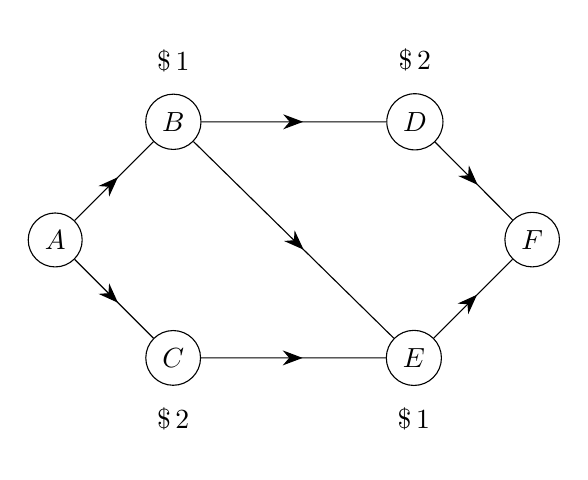
\begin{tikzpicture}[every node/.style={draw,circle}]
            \node (A) at (0,0) {$A$};
            \node[label=above:{$\$\,1$},above right= of A] (B) {$B$};
            \node[label=below:{$\$\,2$},below right= of A] (C) {$C$};
            \node[draw=none,right= of B] (Bempty) {};
            \node[label=above:{$\$\,2$},right= of Bempty] (D) {$D$};
            \node[draw=none,right= of C] (Cempty) {};
            \node[label=below:{$\$\,1$},right= of Cempty] (E) {$E$};
            \node[above right= of E] (F) {$F$};
            
            \path [draw,postaction={on each segment={mid arrow}}]
            (A) -- (B)%
            (A) -- (C)%
            (B) -- (D)%
            (B) -- (E)%
            (C) -- (E)%
            (D) -- (F)%
            (E) -- (F)%
            ;
        \end{tikzpicture}
        \parbox{\linewidth}{\captionof{figure}{}}
    \end{center}
\end{subproblem}


\Problem

\begin{subproblem}
    \label{subproblem:MAT-2202-26-09-2017-4a}
    Show that
    \begin{align*}
        x^2 + 2y^2 & \to \min,\\
        x - y & \leq 0, \\
        x^2 + y^2 - 1 & \leq 0,
    \end{align*}
    %
    is a convex optimisation problem.
\end{subproblem}

\begin{subproblem}
    For the optimisation problem in \cref{subproblem:MAT-2202-26-09-2017-4a} write down the
complete Karush-Kuhn-Tucker (also called KKT) conditions. Explain how we can be certain, for this optimisation
problem, that any optimal solution will satisfy the KKT
conditions.
\end{subproblem}

\end{document}